\begin{priprava}{8., 9}{}{Podmnožice}{Osnove logike in teorije množic}{frontalna}{drsnice, projekcija, tabla}


    \section{Podmnožice}
        
    Množica $\mathcal{B}$ je \textbf{podmnožica} množice $\mathcal{A}$, če za vsak element iz
    $\mathcal{B}$ velja, da je tudi element množice $\mathcal{A}$.
    $$ \mathcal{B}\subseteq\mathcal{A}\Leftrightarrow\forall x\in\mathcal{B}\Rightarrow x\in\mathcal{A} $$
            

    \begin{figure}[H]   
        \centering         
                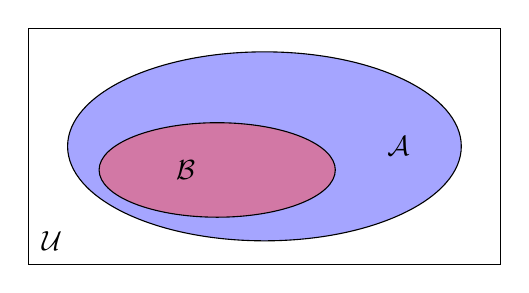
\begin{tikzpicture}                     
                    \draw  (-3,-1.5)  rectangle (3,1.5);
                
                    \draw[fill=blue!70,fill opacity=0.5] (0,0) ellipse (2.5cm and 1.2cm);
                    \draw[fill=red!70,fill opacity=0.5] (-0.6,-0.3) ellipse (1.5cm and 0.6cm);
                    
                    \node at (-1,-0.3) {$\mathcal{B}$};
                    \node at (1.7,0) {$\mathcal{A}$};
                    % \node at (0,1.1) {$\mathcal{B}\subseteq\mathcal{A}$};
                    \node at (-2.7,-1.2) {$\mathcal{U}$};
                    
                \end{tikzpicture}
    \end{figure}


      

        \begin{itemize}
            \item $\forall \mathcal{A}:\mathcal{A}\subseteq\mathcal{A}$ -- Vsaka množica je podmnožica
                same sebe.
            \item $\forall \mathcal{A}:\emptyset\subseteq\mathcal{A}$ -- Prazna množica je podmnožica
                vsake množice. \newline
        \end{itemize}
        

        Moč podmnožice $\mathcal{B}$ množice $\mathcal{A}$ je manjša ali enaka moči množice $\mathcal{A}$:
        $$\mathcal{B}\subseteq\mathcal{A}\Rightarrow m(\mathcal{B})\leq m(\mathcal{A})$$




        Množici $\mathcal{A}$ in $\mathcal{B}$ sta \textbf{enaki}, če imata iste elemente; 
        sta druga drugi podmnožici.
        $$\mathcal{A}=\mathcal{B}\Leftrightarrow(\mathcal{A}\subseteq\mathcal{B})\land(\mathcal{B}\subseteq\mathcal{A})$$

        Podmnožica $\mathcal{B}$ množice $\mathcal{A}$, ki ni enaka množici $\mathcal{A}$, 
        je \textbf{prava podmnožica} množice $\mathcal{A}$.
        \newline

        \textbf{Potenčna množica} množice $\mathcal{A}$ je množica vseh podmnožic množice $\mathcal{A}$.
        
        Oznaka: $\mathbf{\mathcal{P}\mathcal{A}}$ / $\mathbf{\mathcal{P}(\mathcal{A})}$.
        $$ \mathcal{PA}=\left\{\mathcal{X}; \mathcal{X}\subseteq\mathcal{A} \right\}$$
    

        $$ m(\mathcal{PA})=2^{m(\mathcal{A})}$$
        Potenčna množica ni nikoli prazna -- vsebuje vsaj prazno množico.


        ~\\
        \begin{naloga}
            Dana je množica $\mathcal{A}=\{2,4,6,8,10\}$. Zapišite njeno potenčno množico. 
            Kakšna je njena moč?
        \end{naloga}

        \begin{naloga}
            Dana je množica $\mathcal{A}=\{a,b,c,d\}$. Zapiište njeno potenčno množico. 
            Kakšna je njena moč?
        \end{naloga}


\end{priprava}